\documentclass[article]{jss}
\usepackage{amsfonts,thumbpdf}

\newtheorem{lemma}{Lemma}
\newtheorem{theorem}{Theorem}
\newtheorem{corollary}{Corollary}
\newtheorem{example}{Example}
\newtheorem{proposition}{Proposition}
\newtheorem{definition}{Definition}
\newtheorem{conjecture}{Conjecture}
\newtheorem{assumption}{Assumption}
\def\logit{\mathop{\rm logit\,}\nolimits}
\def\midd{\mathop{\,|\,}\nolimits}
\def\defn{{\stackrel{\rm def}{=}}}
\def\eqdistn{{\stackrel{\cal D}{=}}}
\newcommand{\bea}{\begin{eqnarray}}
\newcommand{\eea}{\end{eqnarray}}
\newcommand{\beaa}{\begin{eqnarray*}}
\newcommand{\eeaa}{\end{eqnarray*}}
\newcommand{\qed}{{\rule{2mm}{2mm}}}
\newcommand{\en}{{\rule{.75em}{0cm}}}
\newcommand{\svskip}{\vspace{.125in}}
\newcommand{\mvskip}{\vspace{.25in}}
\newcommand{\lvskip}{\vspace{.5in}}
\newcommand{\R}{\mathbb{R}}

\def\vec#1{\mathchoice{\mbox{\boldmath$\displaystyle\bf#1$}}
{\mbox{\boldmath$\textstyle\bf#1$}}
{\mbox{\boldmath$\scriptstyle\bf#1$}}
{\mbox{\boldmath$\scriptscriptstyle\bf#1$}}}

\title{\pkg{ergmuserterms}: A Template Package}
\Plaintitle{ergmuserterms: A Template Package}
\Shorttitle{\pkg{ergmuserterms}: A Template Package}

\author{
  David R.\ Hunter \\ Penn State University \And
  Steven M.\ Goodreau \\ University of Washington \And
  Mark S.\ Handcock \\ University of Washington 
}
\Plainauthor{David R. Hunter, Steven M. Goodreau, Mark S. Handcock}

\Abstract { 
Abstract here
}
\Keywords{
exponential-family random graph model, Markov chain Monte Carlo, maximum likelihood estimation, p-star model}

%\Volume{}
%\Issue{}
%\Month{}
%\Year{}
%\Submitdate{}
%\Acceptdate{}

\Address{
David R.\ Hunter \\
Department of Statistics \\
Pennsylvania State University \\
University Park, PA 16802, United States of America\\
E-mail: \email{dhunter@stat.psu.edu} \\
URL: \url{http://www.stat.psu.edu/~dhunter/}
}

\begin{document}

\section{Introduction}
\label{introduction}

At the core of the \pkg{ergm} package \citep{ergm} is a sophisticated 
Markov chain Monte Carlo engine for simulating random networks.  
As explained by \citet{ergmjss}, simulating a Markov chain on a
set of networks 
whose stationary distribution is given
by the exponential-family random graph model
\bea\label{ergm}
P_{\vec\theta_0} (\vec Y = \vec y) = 
\frac{ \exp\{ \vec \theta_0^t \vec g(\vec y) \} }
{ \kappa(\vec\theta)}
\eea
is vitally important not only for simulation but also for estimation.
In equation (\ref{ergm}), $\vec\theta_0\in \R^p$ is a fixed parameter vector,
$\vec g(\vec y)$ is a user-defined $p$-vector of statistics on the
network $\vec y$, and 
\beaa
\kappa(\vec\theta) = \sum_{\vec z \in {\cal Y}} \exp\{ \vec \theta_0^t \vec g(\vec z) \}
\eeaa
is the normalizing constant.

{\em Now explain change statistics and why MCMC is dependent on them}

\section[Network storage in ergm]{Network storage in \pkg{ergm}}

A network with $n$ nodes is
internally represented in \pkg{ergm} as a set of $2n$ edgelists, 
$n$ for ``in-edges'' and $n$ for ``out-edges''.  If the directed edge $(3,5)$ exists in the network,
then we call 3 the ``head'' node and 5 the ``tail'' node of this edge.  We would say that node 5 is
on an out-edge from node 3 and that node 3 is on an in-edge to node 5.  Thus, the 3rd out-edge list
should contain 5 and the 5th in-edge list should contain 3.  Naturally, this scheme results in 
redundancy, and maintaining these two sets of edgelists entails both a storage and a performance
cost.  However, in situations where an algorithm must be able to look up both all in-edges and all
out-edges of a node, this scheme is very efficient.  
In the case of an undirected network, the designations of ``head'' and ``tail'' are arbitrary, and we
define the smaller-numbered node as the head and the larger-numered node as the tail.  

Storage of each node's in-edge list and out-edge list is implemented using a standard
binary tree structure
as in \cite[Chapter 13]{algorithms}.  This structure allows for efficient lookup, insertion, and deletion
operations that typically take $O(\log d)$ time, where $d$ is the degree, or number of neighbors, a
particular node has.  In a binary tree such as those shown in Figure \ref{outedgefig},
each parent node has two potential children, with the left child's value always less than the
parent's and the right child's value always greater.  To avoid the worst-case performance
that can result from a list of values being passed in strictly increasing or decreasing order,
each node's edgelist should be randomly permuted before it is stored as a tree.

\begin{figure}[htb]
\vspace{3ex}
$\displaystyle{\pmatrix{
 0 & 0 & 1 & 0 & 0 & 1 & 0 & 1 \cr
 0 & 0 & 0 & 0 & 1 & 0 & 0 & 0 \cr
 0 & 0 & 0 & 0 & 0 & 1 & 1 & 1 \cr
 0 & 1 & 0 & 0 & 1 & 0 & 1 & 0 \cr
 1 & 1 & 1 & 1 & 0 & 0 & 0 & 0 \cr
 1 & 1 & 0 & 0 & 0 & 0 & 0 & 1 \cr
 0 & 0 & 0 & 0 & 0 & 0 & 0 & 0 \cr
 1 & 0 & 1 & 0 & 1 & 0 & 0 & 0 }
 }\qquad\qquad\vtop{\vskip-15ex \hbox{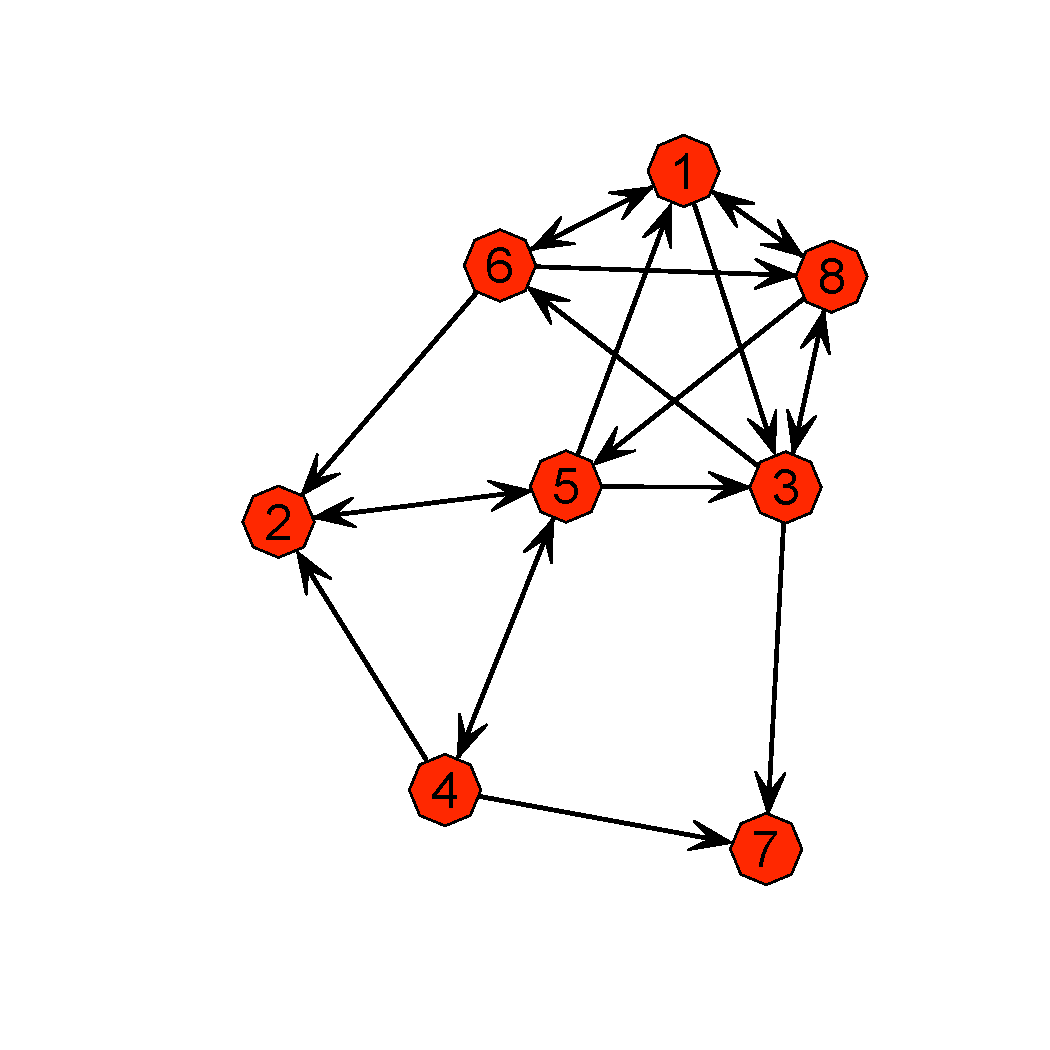
\includegraphics[height=2in, width=2in]{net8nodes.pdf}}}
$
\caption{The adjacency matrix (on left) and a corresponding graphical representation
of a directed 8-node network.  The rows of the adjacency matrix become
the out-edge lists of Figure \ref{outedgefig}.}\label{8nodeexample}
\end{figure}

\begin{figure}[htb]
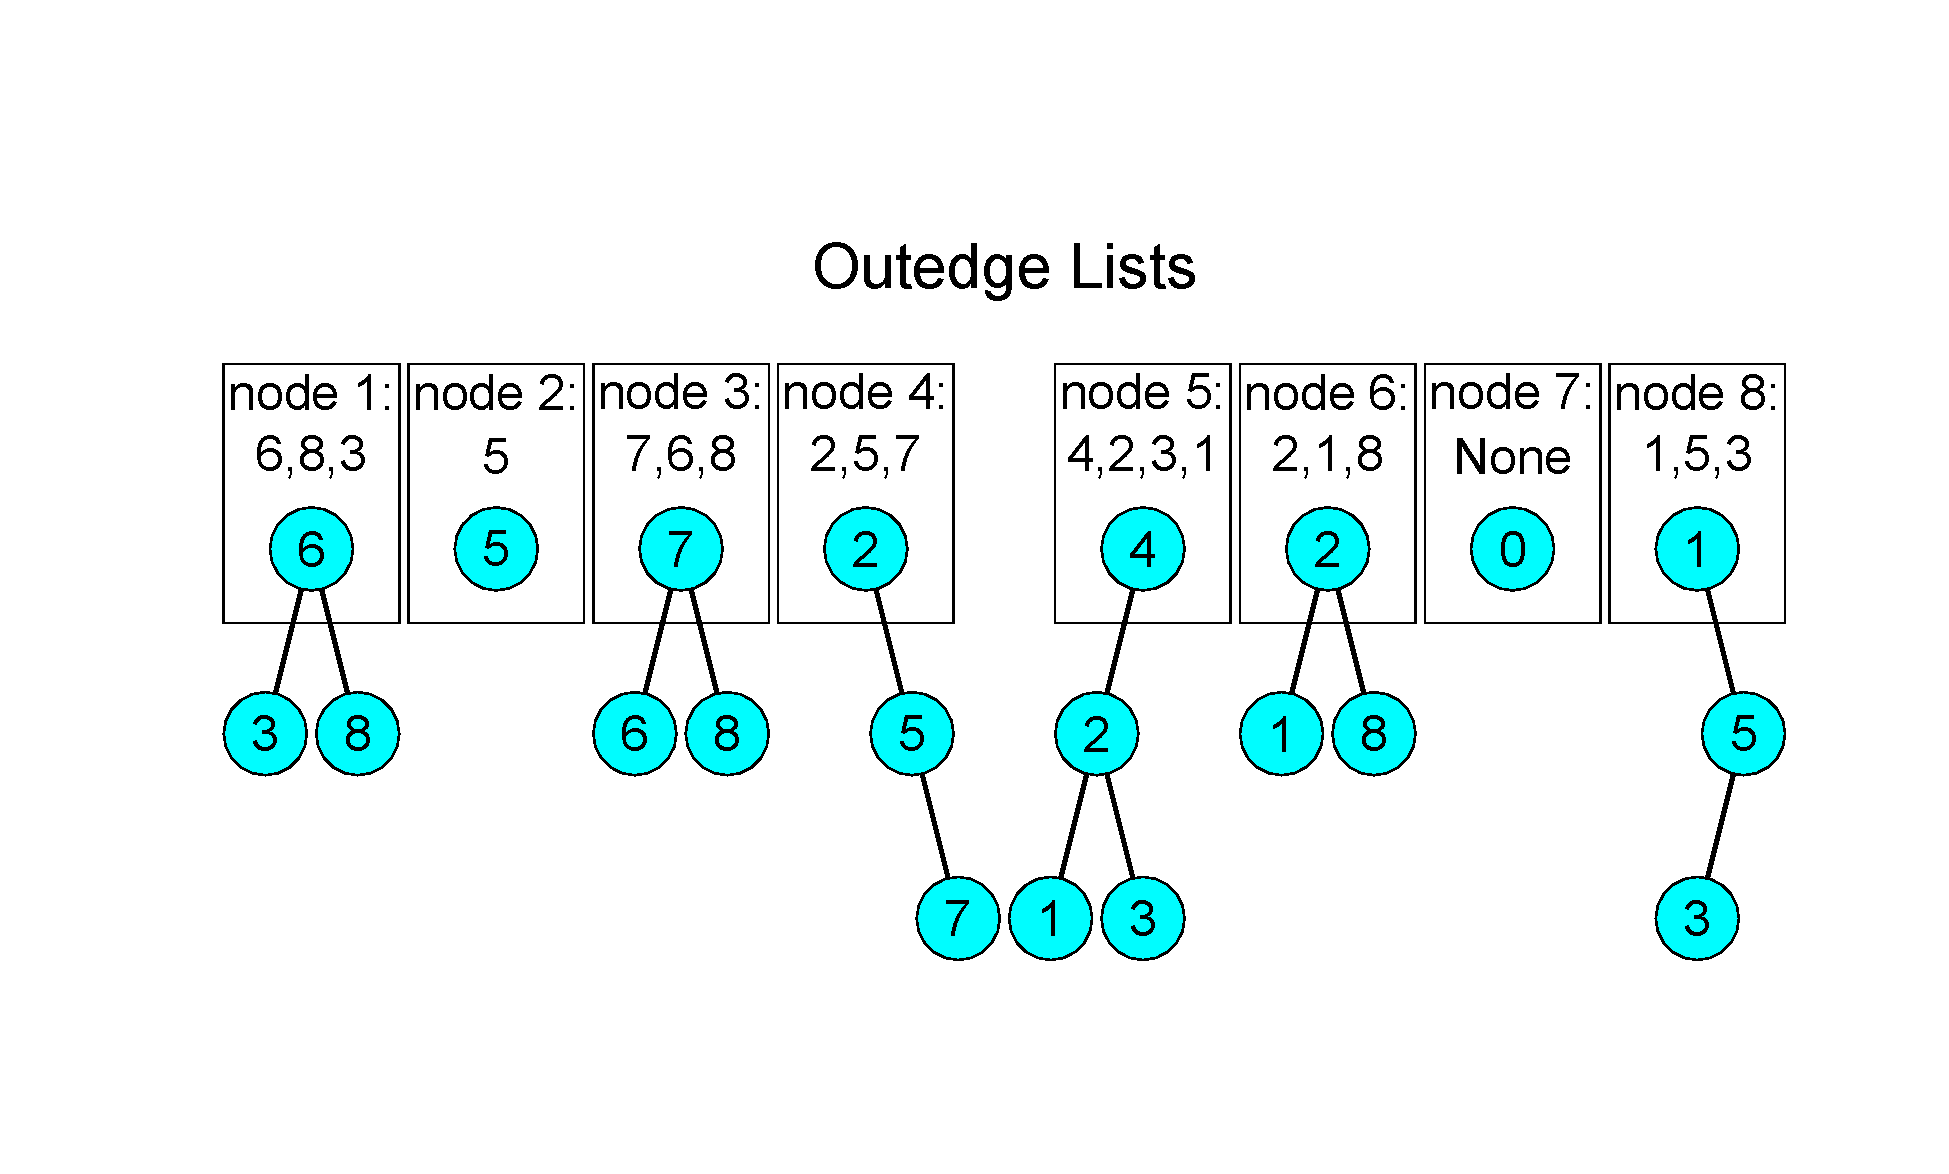
\includegraphics[height=2in, width=4in]{outedgelists.pdf}
\caption{This is the resulting internal representation of the out-edges for the network of
Figure \ref{8nodeexample}.  Each node's out-neighbors are permuted randomly 
before the binary trees are built.}\label{outedgefig}
\end{figure}

The binary tree routines, all written in the C language, are contained in the 
\code{src/edgetree.c} file in the \pkg{ergmterms} package (the \pkg{ergm} package
includes the same code).  These routines may be used to initialize or destroy
a network object, to manipulate that object by adding or deleting edges, and to
query that object to ascertain the presence of an edge.
The \code{NetworkInitialize} and \code{NetworkDestroy} functions 
are used internally by the \pkg{ergm} package to create a network object 
and destroy it when it is no longer needed by the C code.  These two functions
are not generally called by the user, though interested users may find it interesting
to look at them.  Also, the definition of the \code{Network} type, in the 
\code{src/edgetree.h} file, reveals that a network keeps updated lists of every node's
in- and out-degree in addition to the actual edges.  A user may exploit these statistics 
when writing code for various change statistics as described in Section \ref{Cside}.


\section[Writing change statistics using ergmuserterms:  The R side]%
{Writing change statistics using \pkg{ergmuserterms}:  The R side}
\label{Rside}

\section[Writing change statistics using ergmuserterms:  The C side]%
{Writing change statistics using \pkg{ergmuserterms}:  The C side}
\label{Cside}

EdgeTreeSearch
ToggleEdge
AddEdgeToTrees
DeleteEdgeFromTrees
EdgeTreeMinimum
EdgeTreeSuccessor





\section*{Acknowledgments}



\bibliography{v24}

\newpage

\begin{appendix}


\section[appendix]{Appendix}
\label{appendix}

\end{appendix}

\end{document}
